\section*{Method and Setup}\label{sec:ch3_method_setup}

\subsection*{Flow configuration and experimental setup}
Measurements are conducted on the flowpath detailed in \cite{LieberGoyneRockwellEtAl2018a} and depicted in Fig. \ref{fig:ch3_flowpath}. The flow into the scramjet had total temperature 1200 K and total pressure 300 kPa. An immersed insert with in the combustor section hosted a small open cavity flameholder. The cavity had a height $H$ of 3 mm and a closeout ramp angled at 22$^\circ$. The total length $L$ of the cavity from the step to the downstream end of the ramp was 18 mm. This cavity presents a smaller volume of interest for high-fidelity simulations; it was designed so that DNS investigations of the immediate vicinity of the cavity are feasible.  Upstream of the cavity is a short length of constant area duct of height 15 mm, width 38 mm, and length 30 mm with a thin boundary-layer on the cavity side \citep{LieberThesis}. Downstream of the cavity, a 2.9$^\circ$ divergence delays thermal choking. The streamtube captured between the cavity wall of the insert and the opposing wall of the duct merges with the main flow in the main flowpath extender. 

Measurements are acquired in a field of view (FOV) spanning the cavity as shown in Fig. \ref{fig:ch3_FOVs}. The cartesian coordinate system used in the following originates at the center of the cavity leading edge, with $\vec{x}$ along the streamwise axis and $\vec{y}$ along the transverse axis as illustrated in Fig. \ref{fig:ch3_FOVs}.

\begin{figure}[!hbt]
\centering
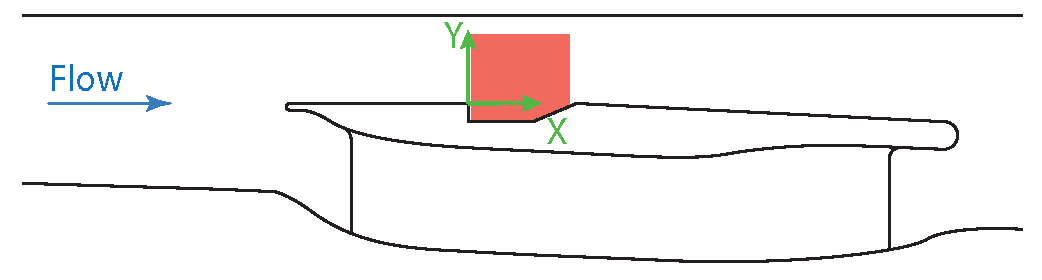
\includegraphics[width=3.25in, trim=0.3in 0in 0.57in 0in, clip]{figures/FOVs/aaArtboard2.png} %pdfcrop
\caption{Field of view of the present work relative to the flameholder.}\label{fig:ch3_FOVs}
\end{figure}

Ethylene fuel is injected from a row of three sonic injectors at 90$^\circ$ to the freestream into the main flowpath isolator to provide a global equivalence ratio of $\Phi_g=0.47$  \cite{RockwellGoyneChelliahEtAl2017}, which corresponds to the highest heat release rate attainable in the facility. The fuel is premixed by the turbulence generated by the isolator shock train. An air throttle at $x/H=57$ provides back pressure; it is set to the minimum flow rate at which combustion stability is maintained. In this configuration, the shock train leading edge is located near near $x/H=-140$. The local Mach number in the combustor was 0.66 (as calculated by a one-dimensional model of the facility isolator \cite{HeiserPrattDaleyEtAl1994}).

\begin{figure*}[!hbt]
\centering
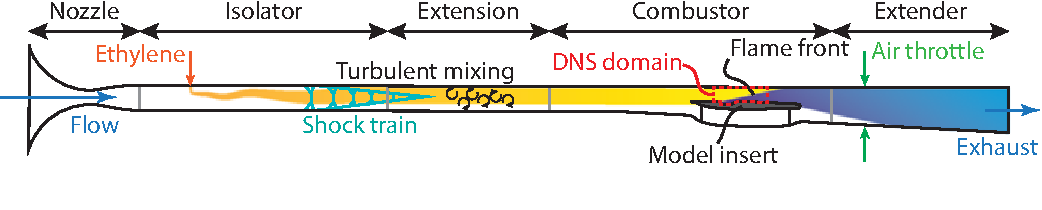
\includegraphics[width=6.5in]{figures/PIV-PLIFsetup/pivplifSmallcavity-crop.pdf} %pdfcrop
\caption{Schematic of the flow path.}\label{fig:ch3_flowpath}
\end{figure*}

The hardware and software system for the PIV-PLIF measurements is illustrated in Fig. \ref{fig:ch3_method_setup}. 
Both the PIV and OH-PLIF measurements are made on the duct spanwise center-plane, relying on the assumption of nominally two-dimensional flow in the cavity, which is consistent with a previous CFD study \cite{ramesh2015large}. The PIV and PLIF systems are run from a common external signal generator. The signal generator is set for the PLIF laser pulse to occur half-way between the two PIV laser pulses as measured by a photodiode. 
The PIV laser is a double-cavity, 10 Hz Spectra Physics PIV-400 Nd:YAG laser delivering two 532 nm-pulses of 500 mJ each, with inter-pulse delays of $\Delta t = 300$ ns. In order to maintain the fluence at the mirrors and model below damage thresholds, 95\% of the energy is dumped using beam splitters. To generate the PLIF laser beam, a Sirah Cobra Stretch dye laser with a mixture of Rhodamine 590 and Rhodamine 610 dyes output a 283.55 nm, 15 mJ/pulse beam to excite the Q$_1$(8) transition of OH \citep{GeipelRockwellChelliahEtAl2017}. The OH-PLIF signal is used as an indicator for the presence of combustion products. The PIV and PLIF laser beams are overlapped using a dichroic filter before the sheet-forming optics. The laser sheet is formed with telescoping optics to a constant height $\sim 25$ mm. To measure the thicknesses of the laser sheets, a portion of each beam was split off after the final focusing lens and was directed through neutral density filters and onto a Point Grey Blackfly CCD camera sensor. The PIV laser sheets are $\sim 140~ \mathrm{\upmu m}$ thick, while the PLIF laser sheet is $75~ \mathrm{\upmu m}$ thick, as measured by full-width at half-maximum at the sheet waist (see Fig. \ref{fig:ch3_meas_LS_thick}). The laser sheets are verified to be coplanar with negligible change in thickness across the FOV.
\begin{figure*}
\centering
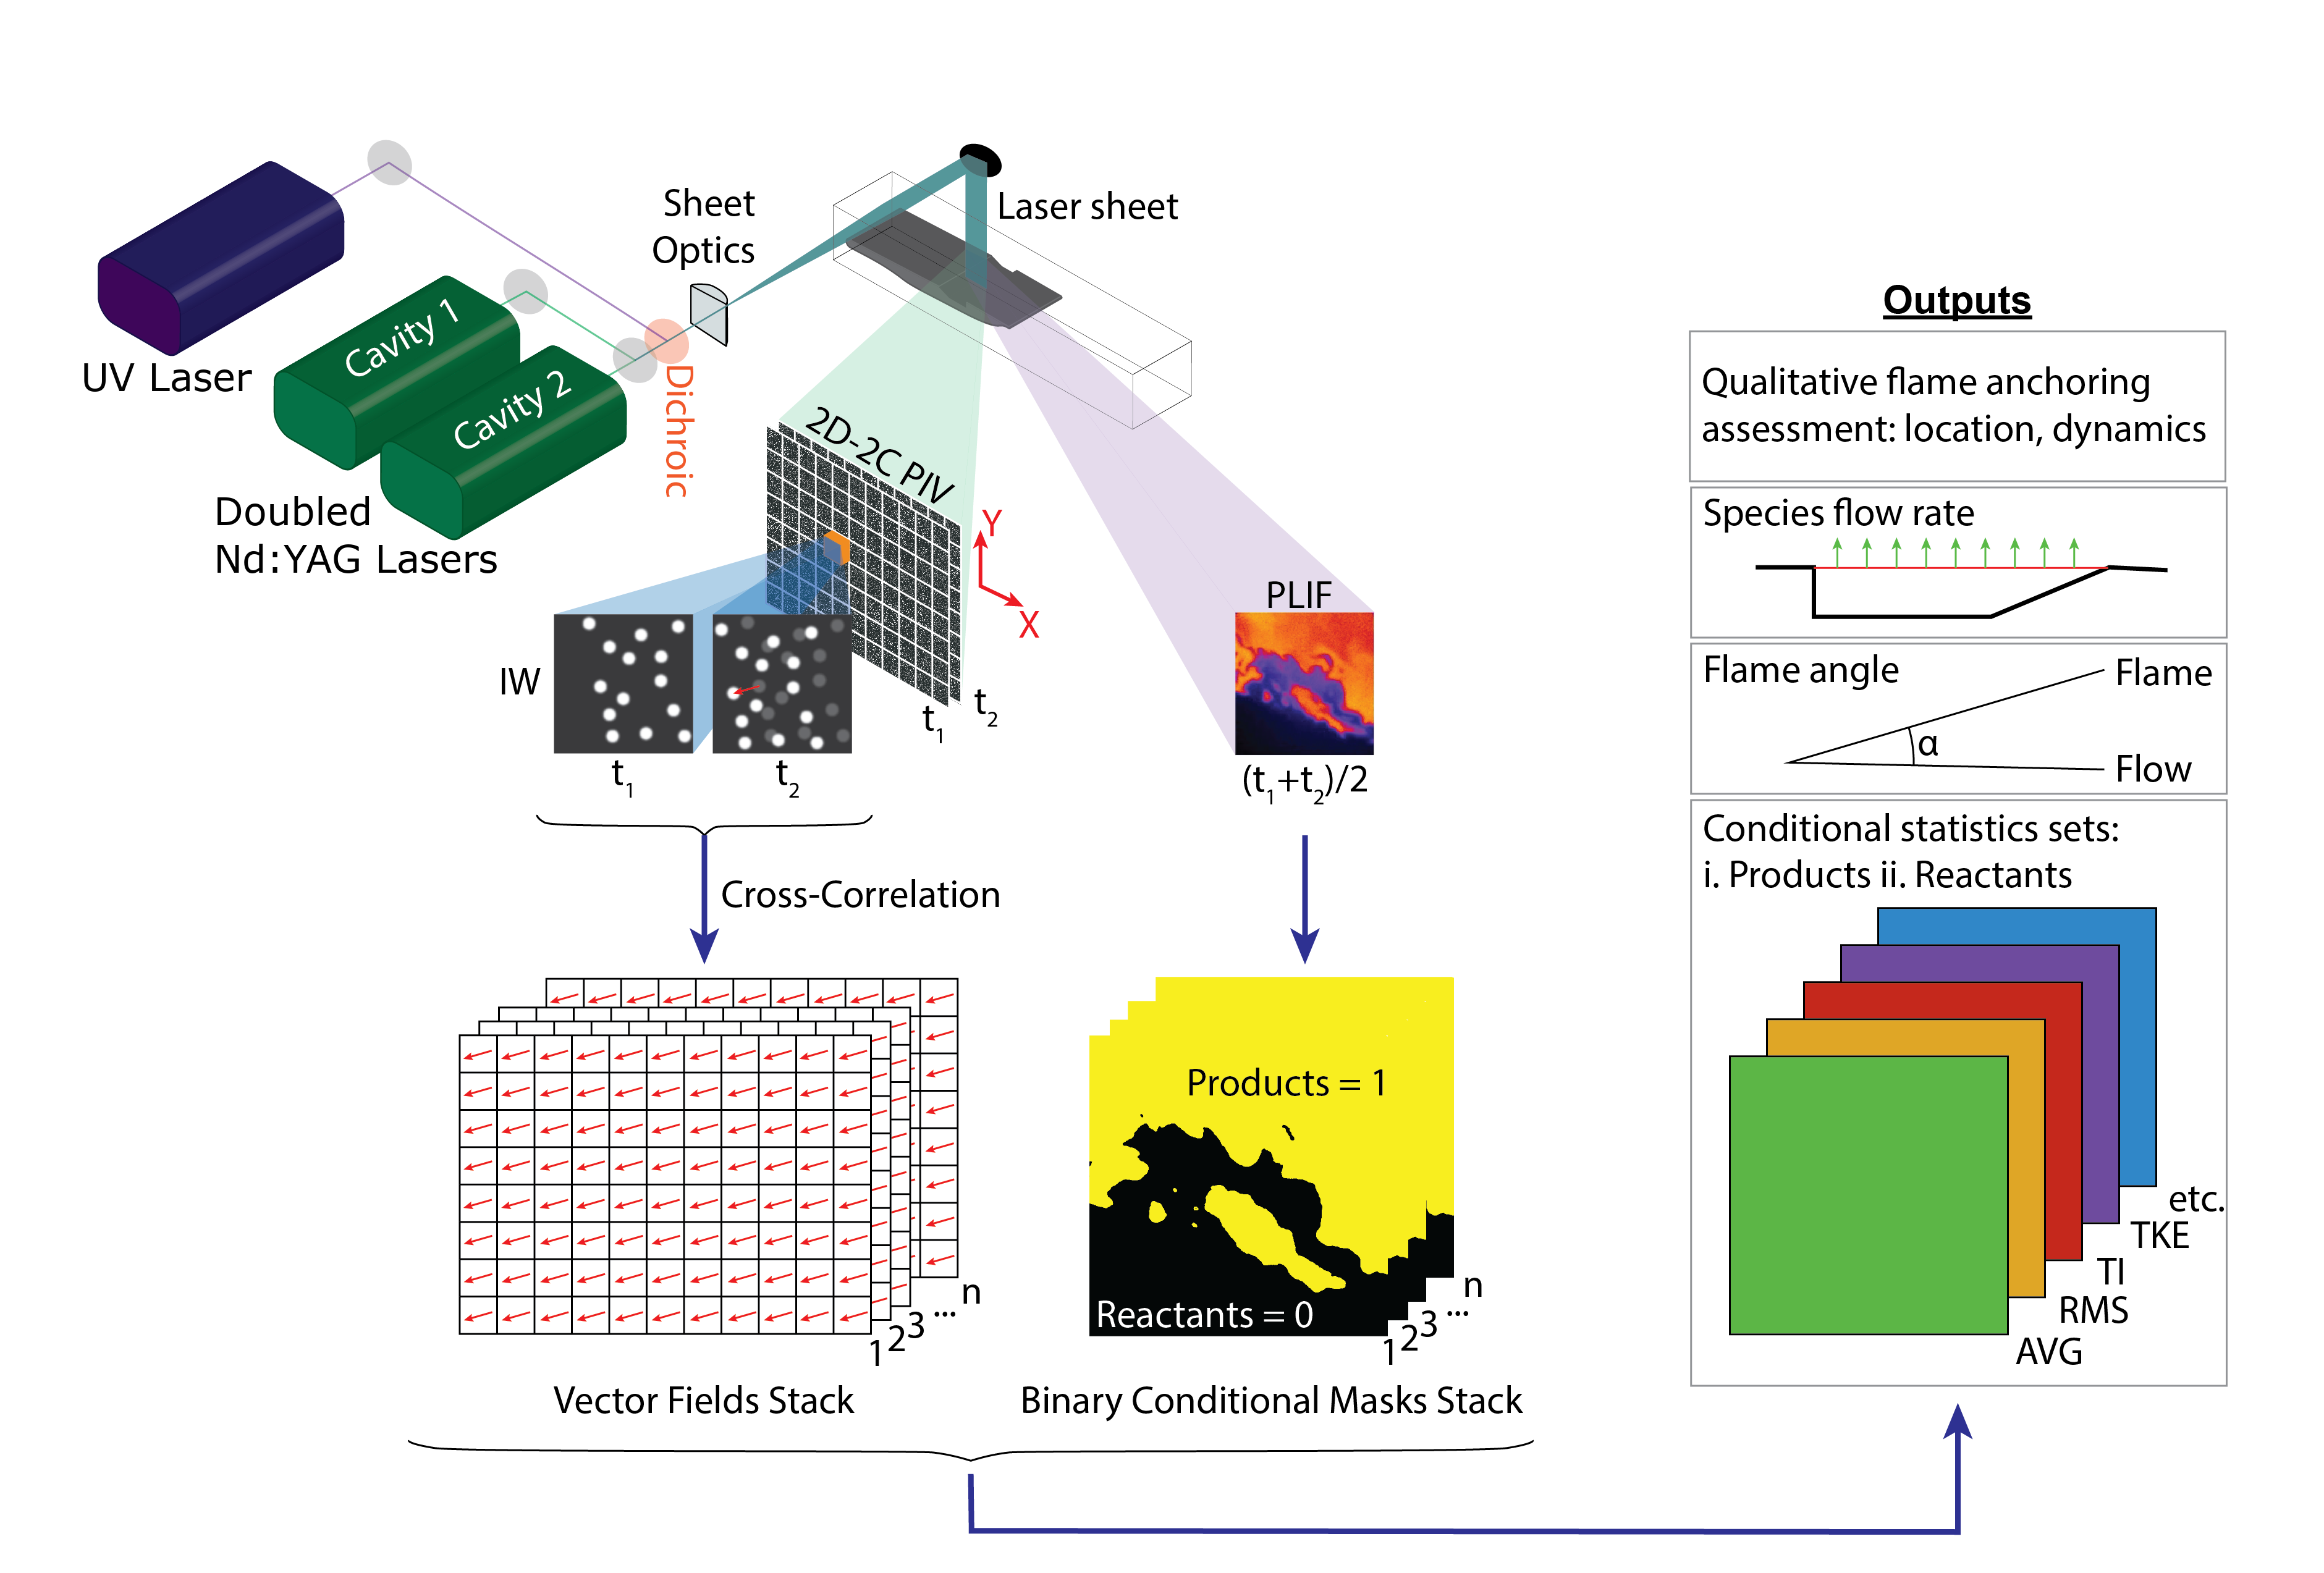
\includegraphics[width=6.5in, trim=0.6in 0in 0.7in 0in, clip]{figures/PIV-PLIFsetup/PIV-PLIFArtboard1@3x.png} %pdfcrop
\caption{Principle of the combined PIV-PLIF technique. AVG: average; RMS: Root-Mean-Square; TI: Turbulence Intensity; TKE: Turbulent Kinetic Energy.}\label{fig:ch3_method_setup}
\end{figure*}

\begin{figure}
\centering
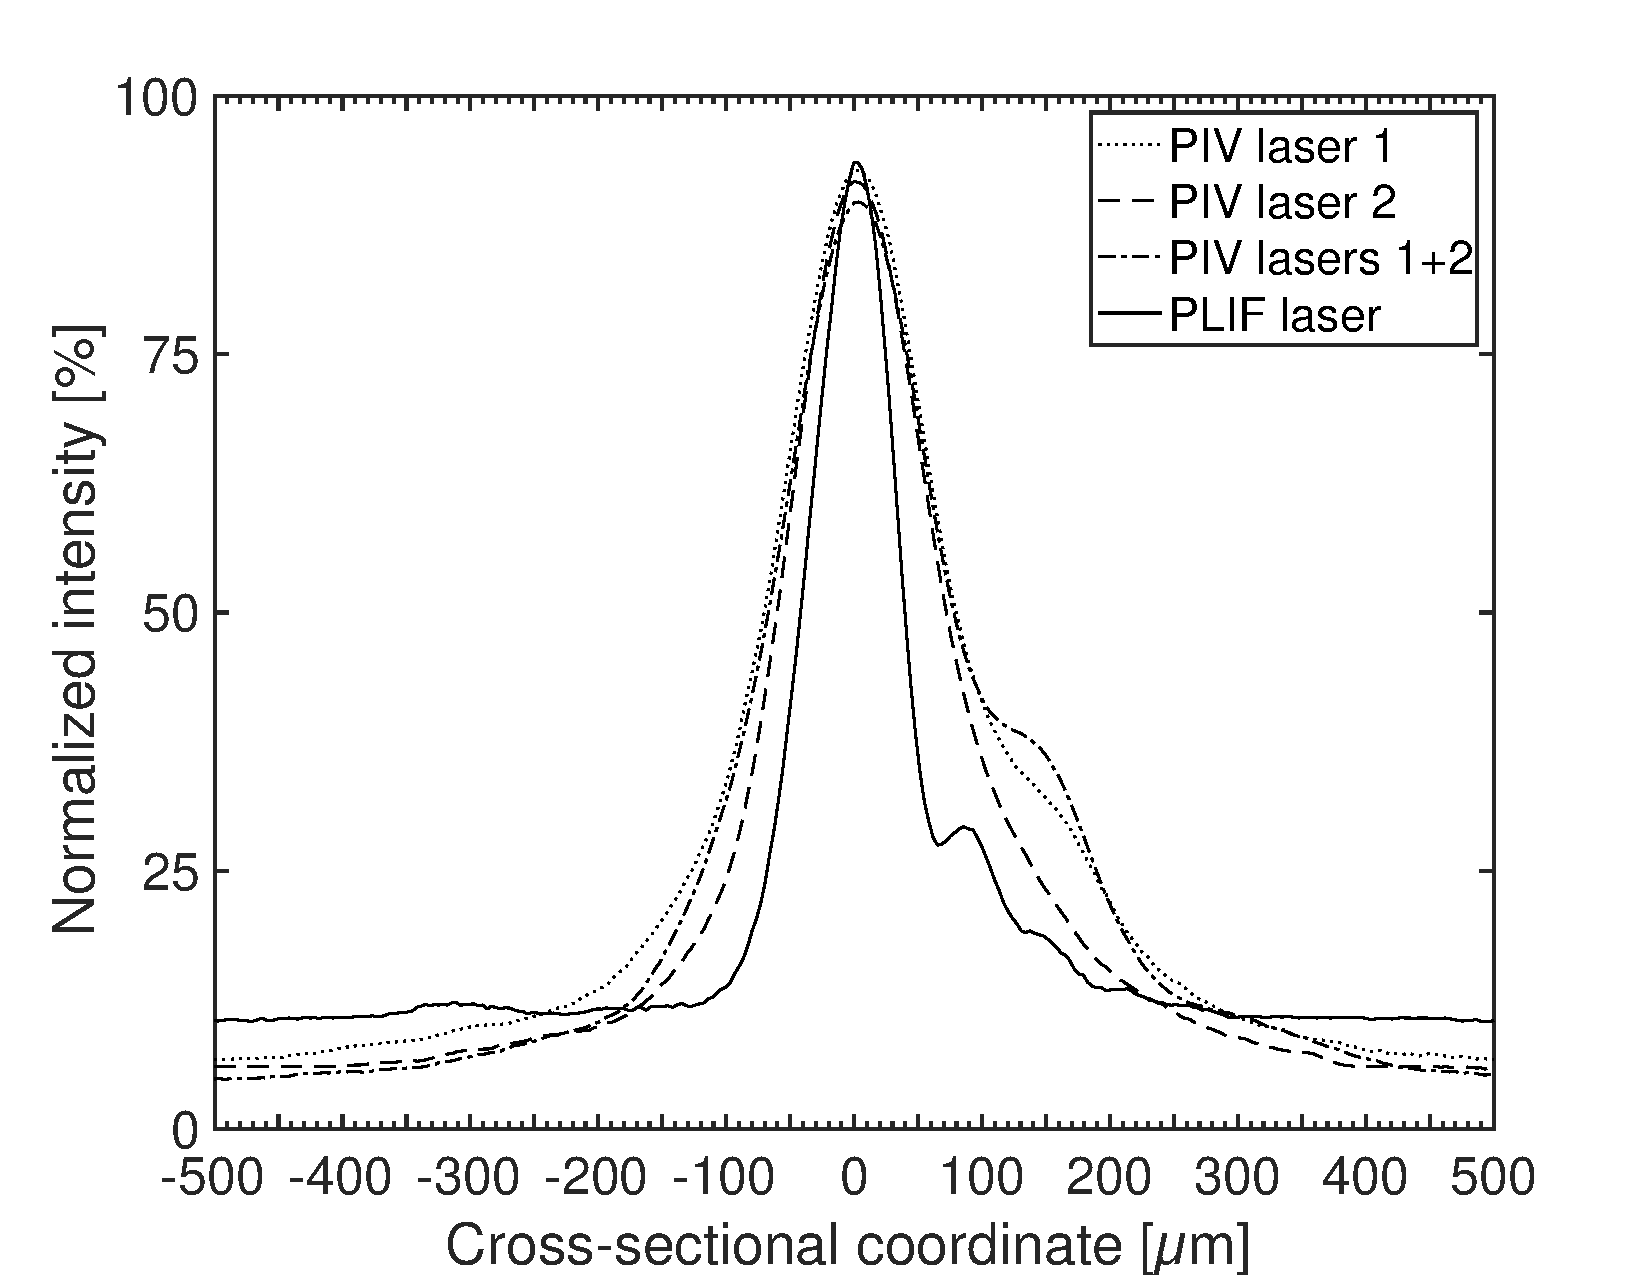
\includegraphics[width=3.25in, trim=0.35in 0in 0.75in 0in, clip]{figures/B_f_overlap_all} %pdfcrop
\caption{Cross-sectional intensity profiles of laser sheets.}\label{fig:ch3_meas_LS_thick}
\end{figure}

The PIV and PLIF cameras are mounted together on a three-axis translational stage system, allowing the field of view to be moved during tunnel operation.
The PIV camera is a 14-bits, $1600\times 1200$ pixel LaVision Imager Pro X 2M. The camera is angled by 4 degrees about the tunnel $x$ axis to mask laser reflections off the wall. A Scheimpflug lens adapter adjusts the focal plane back onto the laser sheet. The camera is mounted with a Micro-Nikkor 105mm f/2.8 lens at a magnification $m=1:1.8$ and an f-number of 11, and a $532 \pm 10$ nm-wide bandpass filter. The lens magnification corresponds to the maximum allowed by the setup constraints; the PIV lens and the PLIF lens would conflict with each other at any higher magnification. The PLIF PI-Max 4 camera is equipped with a 100 mm focal length Cerco lens and a Scheimpflug angle adapter. It captures $512\times 512$ pixel images after $2\times2$ pixel binning. A Semrock FF02-320/40- 30-D bandpass filter reflected light outside the 310-340 nm range \citep{GeipelRockwellChelliahEtAl2017}. 

The PLIF camera is angled by approximately 30 degrees about the tunnel $y$ axis to image the same field of view as the PIV camera. Due to the viewing angle, the region near the cavity ramp is shadowed to the PLIF camera. In addition, the FOV is shifted slightly downstream of the cavity leading edge to avoid imaging laser reflections with the PIV camera, causing clipping of the region immediately behind the cavity backward-facing step. The imaging systems are calibrated simultaneously using a grid with $250~ \mathrm{\upmu m}$ dot spacing. FOV overlap is performed by dewarping and scaling the grid images from both systems before overlapping a spatial marker and all dots across the images. The overlap accuracy is estimated on the order of $10~ \mathrm{\upmu m}$. 

Particle image velocimetry in combusting flows faces challenges that include temperatures greater than 2000 K, wide-spectrum radiation from the flame, and strong gradients in thermo-fluid dynamic variables \citep{StellaGujKompenhansEtAl2001}. This is compounded with the facility high-enthalpy flow, causing the commonly-used PIV tracer materials (e.g. oxides of aluminum, titanium, and silicon ($\mathrm{Al_2O_3}$, $\mathrm{TiO_2}$, $\mathrm{SiO_2}$, \citep{Melling1997, FangHong2018}) to adhere to the facility windows. This adherence quickly prevents flow visualization. 
Kirik et al. \cite{KirikGoyneMcDanielEtAl2017} introduced the use of graphite nano-flakes as tracer particles for the PIV of a cavity flameholder. These $1.1~ \mathrm{\upmu m}$-long and $16~ \mathrm{nm}$-thick flakes have an estimated Stokes number of $St\sim 0.05$ \cite{KirikGoyneMcDanielEtAl2015} corresponding to RMS velocity errors of less than 1\% \citep{SamimyLele1991}. 
Graphite particles prevent window fouling because they do not adhere to the windows as readily. 
Seeding of the graphite nanoflake tracer particles for PIV \citep{KirikGoyneMcDanielEtAl2015} is performed with a fluidized bed seeder \citep{HowisonGoyne2010}. The particles are injected upstream in the isolator, before the fuel injectors and on the centerline. The tracer particles are diffused across the cavity-side streamtube. 

\subsection*{Data processing}
Methodology for PIV processing is presented first, followed by PLIF processing methodology. The graphite nanoflakes used as PIV tracers have a low, angle-dependent reflectance causing poor signal-to-noise ratios. A novel approach solves this problem by pre-processing the images with a Logarithm Contrast-Stretch (LCS) transform, described in \cite{LieberThesis}, in order to compress the upper dynamic range relative to the lower dynamic range. The LCS pre-processing filter increases cross-correlation signal-to-noise ratio in the presence of strong particle image intensity changes between frames. 
The cross-correlation signal-to-noise ratio is also significantly affected by the flame luminosity. Chemiluminescence from the ethylene flame passes through the camera bandpass filter to reach values of 800-8,000 pixel counts depending on the seeding density. This disturbance is particularly severe in the second frame which is constrained by design to a longer exposure time of up to tens of milliseconds depending on the first frame read-out time. A moving average filter across 20 images is thus applied and each frame normalized by the corresponding average before the LCS filter is applied. Lens flares from strong laser reflections off the facility walls are masked before reaching the camera lens.

The data set is then processed with the LaVision DaVis 8.4 cross-correlation algorithm. 
Instantaneous velocities are computed using multi-pass deformed interrogation windows down to 48 $\times$ 48 pixels, corresponding to a velocimetry resolution of $643~ \mathrm{\upmu m}$. Median filters, correlation value thresholds, and outliers detection from temporal distributions remove spurious vectors. Adequate convergence in the velocity mean and RMS is ensured with sample sizes of 1,000 vectors or more. The turbulent kinetic energy (TKE) is estimated by taking the third RMS component as the average of the streamwise and transverse components. The actual three-components turbulent intensity (TI) is on the order of 1\% greater while the TKE is on the order of 100 $\mathrm{m^2/s^2}$ smaller according to a parallel LES study by \cite{Nielsen2019}).
Uncertainties are computed for each instantaneous velocity vector using the measurement signal with the correlation statistics method by \cite{Wieneke2015}, and hardware specifications as detailed in \cite{LieberThesis}. The RMS velocity is corrected by substracting random error fluctuations to isolate flow fluctuations only \citep{SciacchitanoWieneke2016}. 

Processing of the PLIF data is addressed next. The PLIF images are scaled down to $161~ \mathrm{\upmu m/pixel}$ and cropped to match the PIV vector spacing and PIV coordinates. The spatial and temporal resolutions of the PIV measurements are respectively one and five orders of magnitude lower than the estimated Kolmogorov length and time scales. While turbulence spectrum clipping in high $Re$ flows remains inevitable with current technological capabilities, this effect is mitigated for the investigation of turbulence-chemistry interactions: Poinsot et al. \cite{PoinsotVeynanteCandel1991} noted that eddies smaller than the order of the flame front thickness do not quench the flame due to viscous dissipation prior to the flame front. Previous work also demonstrated the dominance of large scale structures in governing the cavity-stabilized combustion process \citep{XavierVandelGodardEtAl2016}. 
The current PLIF technique can only provide qualitative measurements indicative of relative OH concentrations. It is however useful for separating flow regions into reactants- and products-preponderant domains and identifying the location of the flame front \citep{CantuGalloCutlerEtAl2016a}.  An image processing algorithm has been developed to accurately contour the reactants domain; details may be found in \citet{Geipel2019}. 
The image is binarized with one indicating combustion products and zero indicating reactants.  
The binarized PLIF images can be used with the corresponding instantaneous velocities field to output velocities conditioned on both combustion products and reactants (Fig. \ref{fig:ch3_method_setup}). Statistics are finally extracted from the two stacks of velocity fields. The mean transverse velocities across a straight line at $y/H=0$ between the cavity leading and trailing edges, i.e. $x/H=0$ and $x/H=6$, is taken as a representation of the species flux out of the cavity. Mean transverse velocities are similarly estimated at the flame front. 

In the following figures, CLE refers to cavity leading edge. The surface of the tunnel wall opposite to the flameholder is represented by the continuous line at $y/H$ = 4.8 and the insert containing the cavity is shown in grey. A sub-sample of average velocity vectors are displayed with white arrows to show flow directionality. Streamlines in purple originate from each vector.
The flame intermittency is the fraction of instantaneous PLIF measurements in which a significant amount of OH is present at a given location. Intermittency maps are shown as overlayed white contours at the 25\%, 50\%, 75\% and 100\% intermittency levels.
